%-----------------------------------------------------------------------------------------------------
%	INCLUSIÓN DE PAQUETES BÁSICOS
%-----------------------------------------------------------------------------------------------------
\documentclass[a4paper,12pt]{article}
%-----------------------------------------------------------------------------------------------------
%	SELECCIÓN DEL LENGUAJE
%-----------------------------------------------------------------------------------------------------
% Paquetes para adaptar Látex al Español:

%-----------------------------------------------------------------------------------------------------
%	SELECCIÓN DE LA FUENTE
%-----------------------------------------------------------------------------------------------------
% Fuente utilizada.
\usepackage{courier}                    % Fuente Courier.
\usepackage{microtype}                  % Mejora la letra final de cara al lector.
%-----------------------------------------------------------------------------------------------------
%	ALGORITMOS
%-----------------------------------------------------------------------------------------------------
\usepackage{algpseudocode}
\usepackage{algorithmicx}
\usepackage{algorithm}
\usepackage{listings}

%-----------------------------------------------------------------------------------------------------
%	IMÁGENES
%-----------------------------------------------------------------------------------------------------
\usepackage{float}
\usepackage{placeins}
%-----------------------------------------------------------------------------------------------------
%	ESTILO DE PÁGINA
%-----------------------------------------------------------------------------------------------------
% Paquetes para el diseño de página:
\usepackage{fancyhdr}               % Utilizado para hacer títulos propios.
\usepackage{lastpage}               % Referencia a la última página. Utilizado para el pie de página.
\usepackage{extramarks}             % Marcas extras. Utilizado en pie de página y cabecera.
\usepackage[parfill]{parskip}       % Crea una nueva línea entre párrafos.
\usepackage{geometry}               % Asigna la "geometría" de las páginas.
% Se elige el estilo fancy y márgenes de 3 centímetros.
\pagestyle{fancy}
\geometry{left=3cm,right=3cm,top=3cm,bottom=3cm,headheight=1cm,headsep=0.5cm} % Márgenes y cabecera.
% Se limpia la cabecera y el pie de página para poder rehacerlos luego.
\fancyhf{}
% Espacios en el documento:
\linespread{1.1}                        % Espacio entre líneas.
\setlength\parindent{0pt}               % Selecciona la indentación para cada inicio de párrafo.
% Cabecera del documento. Se ajusta la línea de la cabecera.
\renewcommand\headrule{
	\begin{minipage}{1\textwidth}
	    \hrule width \hsize
	\end{minipage}
}
% Texto de la cabecera:
\lhead{\subject}                          % Parte izquierda.
\chead{}                                    % Centro.
\rhead{\doctitle \ - \docsubtitle}              % Parte derecha.
% Pie de página del documento. Se ajusta la línea del pie de página.
\renewcommand\footrule{
\begin{minipage}{1\textwidth}
    \hrule width \hsize
\end{minipage}\par
}
\lfoot{}                                                 % Parte izquierda.
\cfoot{}                                                 % Centro.
\rfoot{Page\ \thepage\ of\ \protect\pageref{LastPage}} % Parte derecha.


%----------------------------------------------------------------------------------------
%   MATEMÁTICAS
%----------------------------------------------------------------------------------------

% Paquetes para matemáticas:
\usepackage{amsmath, amsthm, amssymb, amsfonts, amscd} % Teoremas, fuentes y símbolos.
\usepackage{dsfont} % new fonts added by contributors
\usepackage{tikz-cd} % para diagramas conmutativos
\usepackage[mathscr]{euscript}
\let\euscr\mathscr \let\mathscr\relax% just so we can load this and rsfs
\usepackage[scr]{rsfso}
\newcommand{\powerset}{\raisebox{.15\baselineskip}{\Large\ensuremath{\wp}}}
 % Nuevo estilo para definiciones
\usepackage{hyperref}

%-----------------------------------------------------------------------------------------------------
%	BIBLIOGRAFÍA
%-----------------------------------------------------------------------------------------------------

\usepackage[backend=bibtex, style=numeric]{biblatex}
\usepackage{csquotes}
\usepackage{proof}


\addbibresource{references.bib}

%-----------------------------------------------------------------------------------------------------
%	PORTADA
%-----------------------------------------------------------------------------------------------------
% Elija uno de los siguientes formatos.
% No olvide incluir los archivos .sty asociados en el directorio del documento.
%\usepackage{title1}
\usepackage{title2}
%\usepackage{title3}

%-----------------------------------------------------------------------------------------------------
%	TÍTULO, AUTOR Y OTROS DATOS DEL DOCUMENTO
%-----------------------------------------------------------------------------------------------------

% Título del documento.
\newcommand{\doctitle}{Semester project report}
% Subtítulo.
\newcommand{\docsubtitle}{Internal version}
% Fecha.
\newcommand{\docdate}{}
% Asignatura.
\newcommand{\subject}{}
% Autor.
\newcommand{\docauthor}{Rodrigo Raya Castellano}
\newcommand{\docaddress}{EPFL}
\newcommand{\docemail}{}

%-----------------------------------------------------------------------------------------------------
%	RESUMEN
%-----------------------------------------------------------------------------------------------------

% Resumen del documento. Va en la portada.
% Puedes también dejarlo vacío, en cuyo caso no aparece en la portada.
%\newcommand{\docabstract}{}
\newcommand{\docabstract}{}

 % Teoremas:
\newtheoremstyle{break}
 {\topsep}{10\topsep}%
 {\itshape}{}%
 {\bfseries}{}%
 {\newline}{}%
\theoremstyle{break}

\newtheorem{theorem}{Theorem}[section]  % [section] indica que el contador se reinicia cada sección
\newtheorem{corollary}[theorem]{Corollary} % [theorem] indica que comparte el contador con theorem
\newtheorem{lemma}[theorem]{Lemma}
\newtheorem{proposition}[theorem]{Proposition}

\theoremstyle{break}

\newtheorem*{note}{Note} % * indica que no tiene contador
\newtheorem{construction}{Construction}[section]

% logical formulas:
\newcommand{\func}[1]{\mathrm{#1}}

\newcommand{\qinfer}[3]{%
	\sbox0{\infer{#2}{#3}}%
	\raisebox{\dimexpr(\ht0-1ex)/2}{$#1\;$}%
	\box0
}

\usepackage{mathematics}


\begin{document}

\makeatletter\renewcommand{\ALG@name}{Algoritmo}

\maketitle

%-----------------------------------------------------------------------------------------------------
%	ÍNDICE
%-----------------------------------------------------------------------------------------------------

% Profundidad del Índice:
%\setcounter{tocdepth}{1}

\newpage
\tableofcontents
\newpage

TODO:

Jacobs, Introduction to Coalgebras 

Explains in proposition 2.4.7 how recursion is obtained from induction.

See section 4.6 for references on the construction of final coalgebras. Including Adámeks theorem. Finitary and bounded functors. Relation between coalgebras given with limits and with boundness given by transfinite induction.

Reference for iterative things: Milius, S.: Completely iterative algebras and completely iterative monads

 J. Worrell. On the final sequence of a finitary set functor for the relation between the bounded and the colimit theorems.
 

 
 
\section{The Isabelle architecture and tactics}

We will try a feeling of Isabelle's architecture. To fully address this problem the natural way is to connect the Isar language in which users write proofs with the actual ML level of the system. The reason is that any practical reasoning today happens in this level. On the other hands, only specific proof procedures happen in the ML level. We will try thus to give a reference in which we continue the work begun at EPFL on LCF provers. It is also natural to do it this way to connect the user experience with the actual system experience. Isabelle is big and old. Which means there are lessons to learn. Although is hard to get them.

\subsection{Programming in ML}

Isabelle/ML is based on Poly/ML 1 and thus benefits from the source-level
debugger of that implementation of Standard ML. (reference manual on jedit).

\subsubsection{Datatype declarations}

\begin{lstlisting}
datatype person = King	
		| Peer of string*string*int
		| Knight of string
		| Peasant of string;
\end{lstlisting}

Polymorphic datatype:

\begin{lstlisting}
datatype 'a option = NONE | SOME of 'a
\end{lstlisting}


\subsection{Isabelle/Isar}

The main objective of Isar foundations is to turn existing formal logic concepts (natural deduction, minimal HOL, higher-order resolution and higher-order unification) into  a  viable  language  environment  for  natural  deduction  proof  texts (using concepts from high-level programming languages, leaving behing raw logic). The Isar/VM interpreter connects these two worlds.

Material for Isar: http://isabelle.in.tum.de/Isar/

\subsubsection{Outer\_Syntax and Toplevel}

Clicking at the Isar command we get this value:

\begin{lstlisting}
Outer_Syntax.command ("theory")  "begin theory"
	(Thy_Header.args >> (fn _ => Toplevel.init_theory 
		(fn () => error "Missing theory initialization")));
\end{lstlisting}

Here are two elements that define the parsing and collection of data useful for the internal proofs. 

The Outer\_Syntax structure defines the command function as:

\begin{lstlisting}
val command: command_keyword -> string ->
	(Toplevel.transition -> Toplevel.transition) parser -> unit
\end{lstlisting}

This can be understood as a meta-system transition with some functionality already suggested::

1. Produces as a side-effect a Toplevel.transition -> Toplevel.transition
2. Defines a new command relating its syntax and semantics to the given keyword. Notice that at this level a command is just a datatype with basic compiled information:

\begin{lstlisting}
datatype command = Command of
	{comment: string,
	command_parser: command_parser,
	pos: Position.T,
	id: serial};
\end{lstlisting}

3. Creates a basic theory and context, initializing the header of the theory and registers the Toplevel.transition -> Toplevel.transition to the Isar interpreter.
 
The Toplevel structure (see toplevel.ML) seems to take care of the registered data. It provides an internal state with the operations to pack and unpack theories and Proof.contexts on it. The extensibility of Isabelle as a system framework depends on a number of tables, into
which various concepts commands, ML-antiquotations, text-antiquotations, cartouches, can be entered via a late-binding on the fly.

This section is less well-understood than others. Rough reference is the Ecclectic Manual. However:

Can we debug the ML code as in a pure application?

Actually, it seems that file pure\_syn.ML is only charged of the basic syntax. 

\subsubsection{Isar/VM}

The command language has an interpreter (see proof.ML). Our primary concern here is to explain the virtual machine commands

\begin{figure}
	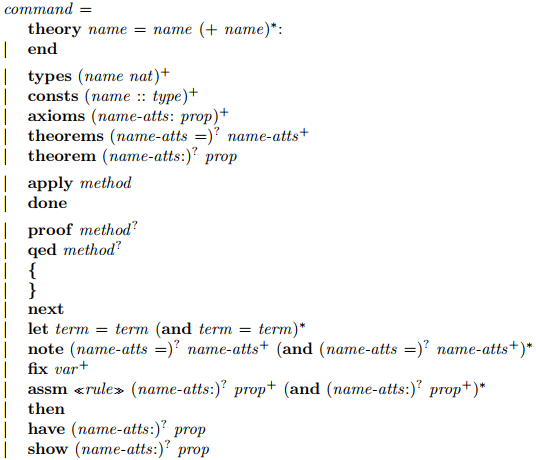
\includegraphics[scale=0.65]{img/commands.png}
\end{figure}












\subsection{Isabelle/HOL}
\subsection{Isabelle/ML}

How do I find out who is using a theory?

\subsection{Learning materials, configurations...}

\subsubsection{Setting up a debugger for ML code}

See chapter 5 of the manual on JEdit. On top of the steps referred there we give the following indications. To activate the plugin just look for the ML debugger option in the plugins folder. It may (in our case it was) be necessary to reload the IDE. To activate the debugger panel, go to Plugins, then Isabelle and then Debugger panel. There should be an option on the option window to dock at the bottom and obtain a similar result to the manual. A minimal example is provided in file Debugger\_Example.thy.

\subsubsection{Exploring finished theories}

See the problem report at StackOverflow:

https://stackoverflow.com/questions/55028386/explore-finished-theories-in-isabelle

In particular we can also 

\subsubsection{Exploring ML files}

How do I explore ML files in a reasonable way? I know of a way to achieve this: you merely need to include your ML file in a *.thy file with the command ML\_file and have both of them open in jEdit. 

\subsubsection{Some examples}

Following:

https://isabelle.in.tum.de/website-Isabelle2019-RC2/dist/library/Doc/Implementation/Proof.html

We do a proof that generalizes 16 different subgoals. Code can be found in ML.

\section{Coinduction}
We propose to study the method of coinduction. We plan to address the following questions:

\begin{itemize}
\item What is coinduction?
\item What are inductive and coinductive definitions. What is recursion and corecursion.
\item Is coinduction as powerful as induction? Or can we prove theorems that could not be proven otherwise?
\item How can coinduction assist automated reasoning and software verification?
\item What kind of complex systems verification would be assisted by coinduction?
\end{itemize}

\subsection{What is coinduction?}

We will schematically show a derivation of the induction and coinduction principles. For details, refer to \cite{rutten} and \cite{leinster}.

Let $F: Set \to Set$ be a functor.

\subsubsection{(Co)algebras}

\begin{definition}[Algebra]
An algebra is a pair $(A,\alpha)$ where $A \in obj(Set)$ and $\alpha \in \mathcal{A}(F(A),A)$.

\begin{center}
\begin{tikzcd}
F(A) \arrow[r, "\alpha"] & A 
\end{tikzcd}
\end{center}
\end{definition}

\begin{definition}[Coalgebra]
A coalgebra is a pair $(A,\alpha)$ where $A \in obj(Set)$ and $\alpha \in \mathcal{A}(A,F(A))$.

\begin{center}
\begin{tikzcd}
A \arrow[r, "\alpha"] & F(A) 
\end{tikzcd}
\end{center}
\end{definition}

One readily observes that algebra and coalgebra are dual notions.

\begin{example}[Peano view of natural numbers]
	$(\mathbb{N},[zero,succ])$ is an $N$-algebra considering the following structure:
	
	\begin{itemize}
		\item $N: Set \to Set$ is a functor such that $N(X) = 1+X$ where $1 = \{*\}$.
				
		Naturally for $f: X \to Y$, $N(f): 1+X \to 1 + Y$ is given as $N(f) = id + f$.
		
		\item $[zero,succ]: 1+\mathbb{N} \to \mathbb{N}$ is a morphism given by:
		
		 $[zero,succ](n) = 
		 \begin{cases}
		 0 & n = * \\
		 succ(n) & n \neq *
		 \end{cases}$
	\end{itemize}
\end{example}	

\begin{example}[Streams as coalgebras]
	$(\mathbb{N}^{\omega}, \langle \operatorname{head}, \operatorname{tail} \rangle)$ is an $Str$-coalgebra considering the following structure:
	
	\begin{itemize}
		\item $Str: Set \to Set$ is a functor such that $Str(X) = \mathbb{N} \times X$.
		
		Naturally for $f: X \to Y$, $Str(f): \mathbb{N} \times X \to \mathbb{N} \times Y$ is given as $Str(f) = id \times f$.
		
		\item $\langle \operatorname{head}, \operatorname{tail} \rangle: \mathbb{N} \to \mathbb{N} \times \mathbb{N}^{\omega}$ given by:
		
		 $\langle head,tail \rangle(\sigma) = (\sigma(0), \sigma(1) \ldots )$
	\end{itemize}
\end{example}

\subsubsection{Relations between (co)algebras}

We relate two (co)algebras via homomorphisms.

\begin{definition}[Homomorphism of algebras]
Given two F-algebras $(A,\alpha),(B,\beta)$. 

An homomorphism $f$ is a morphism making this diagram commute:	
	
\begin{tikzcd}
F(A) \arrow[d, "\alpha"] \arrow[r, "F(f)"] & F(B) \arrow[d, "\beta"] \\
A \arrow[r, "f"] & B 
\end{tikzcd}
\end{definition}

\begin{definition}[Homomorphism of coalgebras]
Given two F-coalgebras $(A,\alpha),(B,\beta)$.

An homomorphism $f$ is a morphism making this diagram commute:	
	
\begin{tikzcd}
A \arrow[d, "\alpha"] \arrow[r, "f"] & B \arrow[d, "\beta"] \\
F(A) \arrow[r, "F(f)"] & F(B)
\end{tikzcd}
\end{definition}

\subsubsection{Categories of (co)algebras}

\begin{definition}[Categories of (co)algebras]
	$Set^F$ is the category of $F$-algebras:
	
	\begin{itemize}
		\item $obj(Set^F)$ is the class of all $F$-algebras.
		\item $\mathcal{A}(A,B)$ are the $F$-homomorphisms between $F$-algebras $A$ and $B$.
	\end{itemize}

	$Set^F$ is the category of $F$-coalgebras:

	\begin{itemize}
		\item $obj(Set_F)$ is the class of all $F$-coalgebras.
		\item $\mathcal{A}(A,B)$ are the $F$-homomorphisms between $F$-coalgebras $A$ and $B$.
	\end{itemize}
\end{definition}

The notion of subobject translates in this context to the following definition:

\begin{definition}[Subalgebras]
	Let $\mathcal{A} = (A,s)$ be an $F$-algebra and $S \subseteq A$. 
	
	The set $S$ together with a morphism $\beta_S:F(S) \to S$ is a subalgebra if the inclusion $i: S \to A$ is an homomorphism. 
\end{definition}

\subsubsection{Initial algebras and terminal coalgebras}

\begin{definition}[Initial algebra/terminal coalgebra]
	An initial algebra is an initial object in $Set^F$. \\
	A terminal coalgebra is a terminal object in $Set_F$.
\end{definition}

\begin{corollary}
	If an initial F-algebra exists it is unique up to isomorphism. \\
	If a final F-coalgebra exists it is unique up to isomorphism.
\end{corollary}
\begin{proof}
	Consequence of the uniqueness of initial and final objects in a category.
\end{proof}

\begin{example}
$(\mathbb{N},[zero,succ])$ is an initial $N$-algebra.\\
$(\mathbb{N}^{\omega}, \langle \operatorname{head}, \operatorname{tail} \rangle)$ is a final $Str$-coalgebra.
\end{example}

The structure map for initial algebras or final coalgebras is an isomorphism:

\begin{lem}[Lambeck]
The structure map of an initial (final) algebra (coalgebra) is an isomorphism.
\end{lem}
\begin{proof}
The idea is to relate the initial algebra $(A,\alpha)$ with the algebra $(F(A),F(\alpha))$.

\begin{tikzcd}
F(A) \arrow[d, "\alpha"]  & F(F(A)) \arrow[d, "F(\alpha)"] \arrow[l, "F(\alpha)"] \\
A  & F(A) \arrow[l, "\alpha"]
\end{tikzcd}

We then exploit initiality to complete the diagram with some $\beta$:

\begin{tikzcd}
F(A) \arrow[d, "\alpha"] \arrow[r,dashed, "F(\beta)"] & F(F(A)) \arrow[d, "F(\alpha)"] \arrow[l, "F(\alpha)"] \\
A \arrow[r,dashed, "\beta"]  & F(A) \arrow[l, "\alpha"]
\end{tikzcd}

From the first diagram $\alpha$ is an homomorphism of algebras. From the second diagram we see that it must be an isomorphism. Indeed, $\beta \circ \alpha$ is a morphism of algebras with domain and codomain in $A$. Again, by initiality, there can only be one such morphism. But the identity is always a morphism. So, $\beta \circ \alpha = id_A$. 

Finally, $\alpha \circ \beta = F(\beta) \circ F(\alpha) = F(\beta \circ \alpha) = F(id_A) = id_F(A)$ looking at the second diagram.
\end{proof}

\begin{cor}[A functor without initial algebras or final coalgebras]
	The (covariant) powerset functor $\mathcal{P}: Set \to Set$ given by:
	
	\begin{itemize}
		\item For each $X \in Set$, $\mathcal{P}(X) = \{U. U \subseteq X\}$.
		\item For each mapping $f:X \to Y$, $\mathcal{P}(f): \mathcal{P}(X) \to \mathcal{P}(Y)$ assigns $U \mapsto f(U)$.
	\end{itemize}
	
	
	does not have initial algebra or final coalgebra.
\end{cor}
\begin{proof}
	Let's assume that $(A,\alpha)$ is an initial algebra (final coalgebra) for $\mathcal{P}$. By Lambek's lemma we know that $\mathcal{P}(A) \cong A$. Isomorphisms corresponds to bijections in $Set$, and thus, $\mathcal{P}(A)$ should be bijective with $A$. This contradicts Cantor's theorem.
\end{proof}

\subsubsection{F-congruences and F-bisimulations}

The second ingredient needed is F-congruences and F-bisimulations:

\begin{definition}[Congruences]
A relation $R \subseteq S \times T$ is an $F$-congruence if there exists an $F$-algebra structure $(R,\gamma)$ such that the projections $\pi_i$ are $F$-homomorphisms:
	
\begin{tikzcd}
F(S) \arrow[d, "\alpha"] & F(R) \arrow[l, "F(\pi_1)"] \arrow[d, "\gamma",dashed] \arrow[r, "F(\pi_2)"] & F(T) \arrow[d, "\beta"]\\
S  & R \arrow[l, "\pi_1"] \arrow[r, "\pi_2"] &  T
\end{tikzcd}
\end{definition}

\begin{definition}[Bisimulations]
A relation $R \subseteq S \times T$ is an $F$-bisimulation if there exists an $F$-coalgebra structure $(R,\gamma)$ such that the projections $\pi_i$ are $F$-homomorphisms:
	
\begin{tikzcd}
S \arrow[d, "\alpha"] & R \arrow[l, "\pi_1"] \arrow[d, "\gamma",dashed] \arrow[r, "\pi_2"] & T \arrow[d, "\beta"]\\
F(S)  & F(R) \arrow[l, "F(\pi_1)"] \arrow[r, "F(\pi_2)"] &  F(T)
\end{tikzcd}
\end{definition}

\subsubsection{(Co)inductive principles}

Introducing the diagonal set may simplify notation:

\begin{definition}[Diagonal]
	The diagonal of a set $A$, is the set $\Delta(A) = \{(a,a). a \in A\}$
\end{definition}

If $R \subseteq A \times A$ then $\Delta^{-1}(R) = \{a \in A. \Delta(a) \in R\} = \{a \in A. (a,a) \in R\}$

The induction and coinduction principles are formulated as follows:

\begin{thm}[Induction proof principle]
	Every congruence relation on an initial algebra contains the diagonal.
\end{thm}

\begin{thm}[Coinduction proof principle]
	Every bisimulation relation on a final coalgebra contains the diagonal.
\end{thm}


Next we give examples on the natural numbers and streams.

Consider the algebra $(\mathbb{N},[zero,succ])$. We will derive the usual induction principle on natural numbers.

\begin{lem}{N-congruence}
	$R$ is an N-congruence relation iff 
	\begin{itemize}
		\item $(0,0) \in R$
		\item $\forall (n,m) \in \mathbb{N}^2. (n,m) \in R \implies (succ(n),succ(m)) \in R$
	\end{itemize}
\end{lem}

\begin{thm}[Induction on natural numbers]
	The principle of mathematical induction:
	
	$\infer{\forall n. P(n)}{%
		P \subseteq \mathbb{N}
		& P(0)
		& \forall n. P(n) \implies P(succ(n)))
	}$
	 
	is equivalent to the N-induction proof principle:
	
	every $N$-congruence relation on $(\mathbb{N},[zero,succ])$ contains $\Delta(\mathbb{N})$
\end{thm}
\begin{proof}
	$ $\newline
	$\Rightarrow)$ Fix a N-congruence relation $R \subseteq \mathbb{N}^2$ and let $P = \Delta^{-1}(R) = \{n \in \mathbb{N}. (n,n) \in R\}$.
	
	We have $(0,0) \in R$ and thus $P(0)$ holds.
	
	Fix $n$ and assume $P(n)$ holds. This means that $(n,n) \in R$ and therefore $(suc(n), suc(n)) \in R$ which implies $P(suc(n))$. 
	
	By the principle of mathematical induction. This means that $\forall n \in \mathbb{N}. (n,n) \in R$ which implies that $\Delta(\mathbb{N}) \subseteq R$. 
	
	$\Leftarrow)$ Fix $P \subseteq \mathbb{N}$ and assume $P(0)$ and $\forall n. P(n) \implies P(succ(n))$.
	
	Define $R = \{(m,n) \in \mathbb{N}^2. P(m) \land P(n)\}$. $R$ is an N-congruence since:
	
	\begin{itemize}
		\item $(0,0) \in R$ as $P(0)$ holds.
		\item $(m,n) \in R \implies P(m) \land P(n) \implies P(succ(m)) \land P(succ(n)) \implies (succ(m),succ(n)) \in R$
	\end{itemize}

	By the N-induction principle, we know that $\Delta(\mathbb{N}) \subseteq R$ and thus, $\forall n. P(n)$ holds.
\end{proof}

We could wonder if the principle of complete mathematical induction:

$\forall P \subseteq \mathbb{N}. (P(0) \land (\forall n. (\forall m < n. P(m)) \implies P(n))) \implies \forall n. P(n)$

also has a categorical interpretation? In any case, it is equivalent to mathematical induction. On the other hand, a direct derivation could be obtained by modifying the predicate $P$ and relation $R$ provided above. 

\begin{lem}
	$R \subseteq \mathbb{N}^{\omega} \times \mathbb{N}^{\omega}$ on $(\mathbb{N}^{\omega}, \langle \text{head}, \text{tail} \rangle)$ is a Str-bisimulation iff:
	
	$\forall (\sigma,\tau) \in R. \text{head}(\sigma) = \text{head}(\tau) \land (\text{tail}(\sigma), \text{tail}(\tau)) \in R$
\end{lem}


\begin{thm}[Coinductive proof principle on Streams]
	The coinductive proof principle applied to the final coalgebra $(A^{\omega}, \langle \text{head}, \text{tail} \rangle)$ takes the following form:
	
	\[
	\infer{s = s'}{%
		R \subseteq A^{\omega} \times A^{\omega}
		& R \; s \; s'
		&
		\qinfer{\forall s_1,s_2}
		{\func{head}(s_1) = \func{head}(s_2) \land R(\func{tail}(s_1), \func{tail}(s_2))}
		{R \; s_1 \; s_2}
	}
	\]
\end{thm}

TODO: An example of proof through coinduction

\subsection{Functional programming and (co)algebras}

Coinduction has been studied in software verification \cite{leino} and theorem proving \cite{blanchette}. We want to explore the implementation of coinduction in Isabelle \cite{blanchette} \cite{sweden}. For that we would like to understand what is a (co)datatype in categorical terms \cite{course} (lecture 8, point 4) \cite{mario}. In this section, we will also investigate how are common functional programming patterns seen from the point of view of category theory.  

\begin{definition}[Polynomial functor]
	Let $A_1, \ldots , A_k$ be sets and $n_1, \ldots n_k \in \mathbb{N}$. 
	
	A functor $F: Set \to Set$ given by: $$F(X) = A_1 \times X^{n_1} + \ldots + A_k \times X^{n_k}$$ is said to be polynomial.
\end{definition}

\begin{remark}
	Interpreted in $Set$, $\times$ is the cartesian product and $+$ is the disjoint union. 
\end{remark}

\begin{definition}[(Co)datatype]
	A datatype is the initial algebra of a polynomial functor. \\
	A codatatype is the final algebra of a polynomial functor.
\end{definition}


Given a polynomial functor $F$ with initial algebra $(T,c)$ where: $$c: A_1 \times T^{n_1} + \ldots + A_k \times T^{n_k} \to T$$ since $+$ corresponds to a disjoint union, we can write $c = [c_1,\ldots,c_k]$ with: $$c_i: A_i \times T^{n_i} \to T$$ Moreover, $T$ is completely determined by the $c_i$ by Lambek's lemma. 

In a programming language, the corresponding constructs are written as follows:

\begin{align*}
datatype \; T &= c_1 \; of \; A_1 \times T^{n_1} \\
&\;\;\vdots \notag \\
&| = c_k \; of \; A_k \times T^{n_k} \\
\end{align*}
\begin{align*}
codatatype \; T &= c_1 \; of \; A_1 \times T^{n_1} \\
&\;\;\vdots \notag \\
&| = c_k \; of \; A_k \times T^{n_k} \\
\end{align*}

\begin{remark}
	The non-categorical interpretation, defines a (co)datatype as the smallest(greatest) set closed by the constructors (destructors).
\end{remark}

\begin{example}[(Co)datatypes by iteration]
	By checking initiality of certain algebras we get to definitions by iteration. 
	
	For instance, let's check that $(\mathbb{N},zs)$ is an initial algebra.
	
	We show that there exists a unique $f$ such that the following diagram commutes:
	
	\begin{tikzcd}
	1 + \mathbb{N} \arrow[r, "N(f)"] \arrow[d, "zs",swap] & 1+X \arrow[d, "\alpha"] \\
	\mathbb{N} \arrow[r, "f",swap] & X
	\end{tikzcd}
	
	That is, $\alpha \circ N(f) = f \circ zs$ where $zs = [zero,succ]$. Equivalently:
	
	\begin{itemize}
		\item $f(0) = \alpha(*)$
		\item $\forall x \in \mathbb{N}. f(x+1) = \alpha(f(x))$ 	
	\end{itemize}

	By natural induction, there is a unique $f$ satisfying this definition.	Since $f$ is defined iterating over $\alpha$, it is sometimes denoted $iter(\alpha)$ \cite{geuvers2007iteration}. More generally, we can see our initial algebra endowed with an iterator mapping $iter$ sending each $\alpha$ to the function $f$ it defines. 
	
	Dually, by checking terminality of certain coalgebras we get definitions by coiteration.
	
	We show that there exists a unique $f$ such that the following diagram commutes:
	
	\begin{tikzcd}
		\mathbb{N}^{\omega} \arrow[d, "ht",swap] & X \arrow[l, "f",swap] \arrow[d, "\alpha"] \\
		\mathbb{N} \times \mathbb{N}^{\omega} & \mathbb{N} \times X \arrow[l, "Str(f)",swap]
	\end{tikzcd}

	That is, $ht \circ f = Str(f) \circ \alpha$ where $ht = [head,tail]$. Equivalently:
	
	\begin{itemize}
	\item $head(f(x)) = \alpha_1(x)$
	\item $tail(f(x)) = f(\alpha_2(x))$ 	
	\end{itemize}

	which defines the stream $f(x) = \alpha_1(x) \; \alpha_1(\alpha_2(x)) \; \alpha_1(\alpha_2^ 2 (x)) \ldots$. Since $f$ is defined iterating over $\alpha$, it is sometimes denoted $coiter(\alpha)$ \cite{geuvers2007iteration}. More generally, we can see our terminal coalgebra endowed with a coiterator mapping $coiter$ sending each $\alpha$ to the function $f$ it defines. 		
\end{example}

It is worth noting from the examples above that the structure map of a (co)algebra indicates the basic operations that are available for the (co)datatype, while the initiality property is essential in proving facts about the (co)datatype. \cite{smyth1982category}

Definitions by iteration provide means of computing functions $f$ starting from an initial value $*$ and then applying iteratively the same function $\alpha$ to the obtained computations. We can also model other definitional paradigms, namely, primitive recursion and case analysis. 

\begin{lemma}[Primitive recursion on initial algebras]
	Let $(A,in,iter)$ be an initial algebra and $g: T(B\times A) \to A$. 
	
	There is a unique morphism $h$ making the following diagram commute:
	
	\begin{tikzcd}
		T A \arrow[d, "in",swap] \arrow[dashed]{r}{T \langle h,id \rangle} & T(B \times A) \arrow[d,"g"] \\
		A \arrow[r, "h",swap, dashed] & B
	\end{tikzcd}

	In fact, $h = \pi_1 \circ iter\langle g, in \circ T(\pi_2)\rangle$
\end{lemma}
\begin{proof}
	See lemma 2.5 in \cite{geuvers2007iteration}.
\end{proof}

\begin{example}[Primitive recursion on natural numbers]
The scheme for primitive recursion on natural numbers looks as follows:

\begin{itemize}
	\item $h(0) = g_1(*)$
	\item $h(succ(n)) = g_2(h(n), n)$ 
\end{itemize}

This can be modeled using $T = N, A = B = \mathbb{N}$. 

The predecessor function is often quoted to be easier to be defined through recursion than by iteration.
\end{example}

Since $h$ is defined recurring to $g$, we write it $h = rec(g)$ and for an initial algebra we can establish a mapping $rec$ assigning to each extra parameter supplier $g$, the function $h$ it defines.

\begin{lem}[Case analysis on initial algebras]
	Let $(A,in,iter)$ be an initial $T$-algebra and $g:T(A) \to B$.
	
	There exists a unique morphism $h$ making the following diagram commute:
	
	\begin{tikzcd}
		T A \arrow[r, "in",swap] \arrow[swap]{dr}{g} & A \arrow[d,"h",dashed] \\
		 & B
	\end{tikzcd}
\end{lem}

\begin{example}[Case analysis on natural numbers]
	Case analysis over natural numbers can be seen as follows:
	
	\begin{itemize}
		\item $h(0) = g_1(*)$
		\item $h(succ(n)) = g_2(n)$
	\end{itemize}

	This corresponds to the above definitions with $T = N, A = \mathbb{N}$.
\end{example}


TODO: corecursion, cocase analysis


\subsection{Building initial and final algebras}

Our goal now is to investigate different approaches to build datatypes and codatatypes in programming language theory. From the examples above it is reasonable to ask the following question: does the initial/final (co)algebra of a polynomial endofunctor always exist? If so, can we compute it?

\subsubsection{Adamek's and Barr's theorems}

We consider a generalization of Kleene's fixed-point theorem. It may be interesting to include some notation so that we understand better the construction involved. 

\begin{thm}[Adamek-Barr]
	The two statements below are dual of each other:
	
	\begin{itemize}
		\item Let $\mathcal{C}$ be a category with initial object $0$ and colimits for any $\omega$-chain. If $F: \mathcal{C} \to \mathcal{C}$ preserves the colimit of initial $\omega$-chain, then the initial $F$-algebra is $\mu(F) = \text{colim}_{n < \omega} F^n 0$.
		\item Let $\mathcal{C}$ be a category with terminal object $1$ and limits for any $\omega^{op}$-chain. If $F: \mathcal{C} \to \mathcal{C}$ preserves the limit of terminal $\omega^{op}$-chain, then the terminal $F$-coalgebra is $\nu(F) = \text{lim}_{n < \omega^{op}} F^n 1$.
	\end{itemize}
	
\end{thm}
\begin{proof}
	We follow here the proof in Jacobs \cite{jacobs2005introduction} who does it for the second case.
	
	Assume there is a limit $Z$ of the chain starting at the final object:
	
	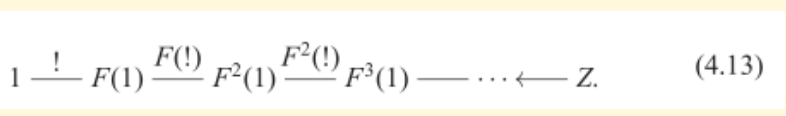
\includegraphics[width=0.5\textwidth]{img/chain}
	
	If $F$ preserves $\omega$-limits then $Z \to F(Z)$ is a final coalgebra.
	
	Actually we only need that $F$ preserves the limit of this chain. 
	
	Assume that $Z$ in the above diagram is a limit with $\xi_n:Z \to F^n(1)$ the corresponding commutative cone satisfying that $F^n(!) \circ \xi_{n+1} = \xi_n$. 
	
	Applying $F$ to the cone and the above equations yields another commutative cone with base $F(Z)$  and components $F(\xi_n):F(Z) \to F^{n+1}(1)$. The limit of this cone is $F(Z)$ since by assumption $F$ preserves limits.
	
	Now, it should be observed that indeed, $Z$ can be used as the base of a shorter cone starting at $F(1)$. Since, $F(Z)$ is the limit of such chain we get a unique homomorphism $\xi: Z \to F(Z)$. 
	
	Incidentally one can also extend the chain whose base is $F(Z)$ into a chain starting in $1$ this is by using the unique properties of terminal object $1$. Commutativity holds and at the end we get another homomorphism $\xi': F(Z) \to Z$. It follows that $\xi \circ \xi'$ and $\xi' \circ \xi$ are homomorphisms on final cones. This implies that they are the identity.
	
	In summary, we can also say that $\xi$ is an isomorphism with inverse $\xi'$. The homomorphism condition yields the equation $F(\xi_n) \circ \xi \stackrel{1}{=} \xi_{n+1}$
	
	Then he goes on to show that $(Z,\xi)$ is a final coalgebra. 
	
	For an arbitrary coalgebra $c:Y \to F(Y)$ we can form a collection of maps $c_n: Y \to F^n(1)$ via:
	
	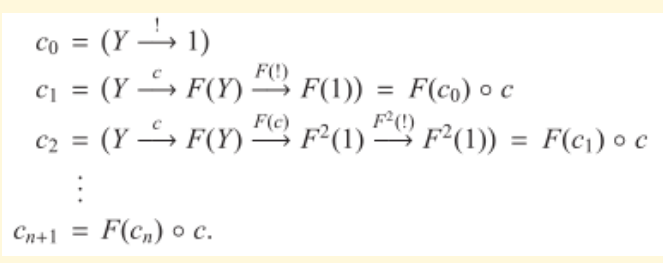
\includegraphics[width=0.5\textwidth]{img/mappings}
	
	The base $Y$ and the maps $c_n$ form a commutative cone. To see this it is useful to distinguish between $!_y$ and $!_1$ which signals to what chain does the unique morphism belong to. By induction:
	
	Base case: $c_0 = !_1 \circ c_1$. This holds directly because of the uniqueness of $c_0 = !_y$. 
	
	Inductive case: let's assume that $c_{n-1} = F^{n-1}(!_1) \circ c_{n}$.  We have to show that $c_{n} = F^{n}(!_1) \circ c_{n+1}$.
	
	Indeed,from the induction hypothesis we get that $F(c_{n-1}) \stackrel{*}{=} F^n(!_1) \circ c_n$ and the right hand side then is:
	
	$F^{n}(!_1) \circ c_{n+1} = F^{n}(!_1) \circ F(c_n) \circ c \stackrel{*}{=} F(c_{n-1}) \circ c = c_n$
	
	As a consequence, since $Z$ is the base of the initial cone this yields a unique cone homomorphism $h: Y \to Z$ with $\xi_n \circ h \stackrel{3}{=} c_n$
	
	
	Let's check that $h$ is an homomorphism of coalgebras, i.e satisfies $\xi \circ h = F(h) \circ c$.
	
	Note at this point that while $\xi \circ h$ is a cone homomorphism, it is not necessary the case that $F(h) \circ c$ is. In particular, we don't have that $c$ is a cone homomorphism.
	
	We would be done if we check that both behave the same on the components of the cone with base $F(Z)$. This would imply that $F(h) \circ c$ is also an homomorphism. Since $F(Z)$ is a limit there can be only one such homomorphism and the equality follows. Now:
	
	$F(\xi_n) \circ \xi \circ h \stackrel{1}{=} \xi_{n+1} \circ h \stackrel{3}{=} c_{n+1} \stackrel{2}{=} F(c_n) \circ c \stackrel{3}{=} F(\xi_n) \circ F(h) \circ c$
	
\end{proof}

\begin{cor}
	Any polynomial functor on $Set$ admits an initial algebra and a final coalgebra.
\end{cor}
\begin{proof}
	Check with corollary 4.6.3 in \cite{jacobs2005introduction}.
\end{proof}


In the context of Isabelle these constructions are however, not suited because arbitrary limits require reasoning about infinite type families which is not available in HOL.


\subsubsection{Bounded endofunctor theorem}


The finite powerset is not continuous but has a final coalgebra. Hence we shall need
more powerful techniques to cover a larger class of functors. 





\section{Coinduction in Isabelle}
What do we have to do?

The user specifies some type constructors. 

'a List = Nil $|$ Cons 'a ('a List) 

this can be understood as a fixed point equations on types:

$X = 1 + A \times X$

the (co)induction package has to derive appropriate theorems for such an equation in a sound way according to the  kernel. So we formulate the following questions:

1. Given such a user definition, how do we derive the functorial 
structure?

2. Given the functorial structure, how do we derive in the logic the
induction and coinduction principles? Introduction rules? Case analysis?
And so on...This is answer by Traytel's AFP entry.

3. How could Stainless produce such (co)inductive principles?

\subsection{Functorial structure}

HOL can be modeled as a category using the universe of types $U$ as objects and functions between types as morphisms. Some useful type constructor $(\alpha_1,\ldots,\alpha_n)F$ correspond then to the notion of functor on $U$. We will rephrase the definition of functor in this context as follows:

\begin{definition}[Type constructors as functors]
	Let $\overline{\alpha}F$ be a type constructor and: $$\text{Fmap}: \overline{\alpha} \to \overline{\beta} \to \overline{\alpha} F \to \overline{\beta} F$$ be a mapping satisfying: 
	
	\begin{itemize}
		\item $\text{Fmap} \; \text{id} = \text{id}$
		\item $\text{Fmap} (\overline{g} \circ \overline{f}) = \text{Fmap} \, \overline{g} \circ \text{Fmap} \, \overline{f}$
	\end{itemize}
	
	Then we say that $(\text{F}, \text{Fmap})$ is a functor whose action on objects is $\text{F}$ and on morphisms is $\text{Fmap}$.
\end{definition}

In Isabelle, (co)datatypes are obtained composing the following basic functors:

\begin{table}[h]
	\begin{center}
		\begin{tabular}{ | l | c | r | }
			\hline
			Name & On objects & On morphisms \\ \hline
			Constant & $C_{\alpha} = \alpha$ & $\text{Cmap}_{\alpha} = id_{\alpha}$  \\ 
			Sum & $+(\alpha_1,\alpha_2) = \alpha_1 + \alpha_2$ & $f_1 \oplus f_2(\text{Inj}_i a) = \text{Inj}_i (f_i \, a)$ \\
			Product & $\times(\alpha_1,\alpha_2) = \alpha_1 \times \alpha_2$ & $f_1 \otimes f_2(x,y) = (f_1(x),f_2(y))$ \\
			Function space & $\text{func}_{\alpha}(\beta) = \alpha \to \beta$ & $\text{comp}_{\alpha} \, f \, (g) = f \circ g$ \\ 
			Powertype & $\text{set}(\alpha) = \alpha \, \text{set}$ & $\text{image}(f)(A) = f(A)$ \\ 
			k-Powertype & $\text{set}_k(\alpha) = \text{typeof } \{A: \alpha \, \text{set}. \text{card}(A) < k\}$ & $\text{image}_k = \text{image} \, f|_{\{A: \alpha \, \text{set}. \text{card}(A) < k\}}$ \\ 
			\hline
		\end{tabular}
	\end{center}
	\caption{Basic functors}
	\label{table:1}
\end{table}

Let's observe how the notion of subalgebra is simplified in this context. Let $(A,t)$ be a $F$-subalgebra of the algebra $(B,s)$. This means that the inclusion $i: A \to B$ is an $F$-algebra homomorphism. In this setting, we can actually state that $F(i) = i$. This simplifies the subalgebra equation to $s \circ i = i \circ t$ which implies that $t = s|_{F(A)}$. 

Here are some examples of the encoding of (co)datatypes using basic functors:

\begin{table}[h]
	\begin{adjustwidth}{-2.5cm}{}
		\begin{center}
			\begin{tabular}{ | l | c | c | c | r | }
				\hline
				Datatype & On objects & On morphisms & (Co)algebra structure & Abstract interface \\ \hline
				Finite lists & $(\alpha,\beta) \text{F} = \text{unit} + \alpha \times \beta$ & $\text{Fmap} \, f \, g = \text{id} \oplus f \otimes g$ & $\text{fld} = \langle \text{Nil}, \text{Cons} \rangle$ & $(\text{list},\text{map})$  \\ 
				FBFD trees & $(\alpha,\beta)F = \alpha \times \beta \; \text{list}$ & $\text{Gmap} \, f \, g = f \otimes \text{map} \, g$ & $\text{fold} = $ & b \\
				FBID trees & $(\alpha,\beta)F = \alpha \times \beta \; \text{list}$ & $\text{Gmap} \, f \, g = f \otimes \text{map} \, g$ & $\text{unf} = \langle \text{lab}, \text{sub} \rangle$ & b \\
				UFBPI trees & $(\alpha,\beta)H = \alpha \times \beta \, \text{fset}$ & $\text{Hmap} \, f \, g = f \otimes \text{fimage} \, g$ & $\text{unf} =$ & d \\
				\hline
			\end{tabular}
		\end{center}
	\end{adjustwidth}
	\caption{Examples of datatypes}
	\label{table:1}
\end{table}

The notion of bounded natural functor, provides the necessary axioms allowing to introduce initial and final coalgebras in HOL:

\begin{definition}[BNF]
	An n-ary bounded natural functor is a tuple $($F, Fmap, Fset, Fbd$)$ where:
	
	\begin{itemize}
		\item $F$ is an n-ary type constructor.
		\item $\text{Fmap}: \overline{\alpha} \to \overline{\beta} \to \overline{\alpha} F \to \overline{\beta} F$
		\item $\forall i \in \{1,\ldots,n\}.$ Fset$_i: \overline{\alpha}F \to \alpha_i \text{ set}$
		\item Fbd is an infinite cardinal number.
	\end{itemize}
	
	satisfying the following:
	
	\begin{itemize}
		\item (F,Fmap) is a binary functor.
		\item Fset$_i: \overline{\alpha}F \to \alpha_i \text{ set}$ is a natural transformation from:
		
		$((\alpha_1,\ldots,\alpha_{i-1},\textunderscore,\alpha_{i+1},\ldots,\alpha_n)F, \text{Fmap})$ to $(\text{set}, \text{image})$.
		\item (F,Fmap) preserves weak pullbacks.
		\item $\forall a \in \text{Fset}_i \, x,  i \in \{1,\ldots,n\}. f_i \, a = g_i \, a \implies \text{Fmap} \, \overline{f} \, x = \text{Fmap} \, \overline{g} \, x$
		\item The following cardinal bound conditions hold:
		
		$\forall x : \overline{\alpha} F, i \in {1,\ldots,n}. |\text{Fset}_i \, x | \le \text{Fbd}$
	\end{itemize}
\end{definition}

The naturality condition generalizes our observation about subalgebras for basic functors to any bounded natural functor. For a BNF, a subalgebra consists of a subset together with a restriction of the structure mapping to the substructure obtained after applying the functor to the subset. This is the so-called shape and content intuition that the authors write in their papers.

\begin{table}[h]
	\begin{adjustwidth}{-2.5cm}{}
		\begin{center}
			\begin{tabular}{ | l | c | r | }
				\hline
				F & Fset & Fbd \\ \hline
				$C_{\alpha}$ & & $\aleph_0$ \\
				$+$ &  & $\aleph_0$ \\
				$\times$ &  & $\aleph_0$ \\
				func$_{\alpha}$ & image g $U_{\alpha}$ & $\max\{|\alpha|,\aleph_0\}$  \\
				set$_k$ & & max$\{k,\aleph_0\}$ \\
				\hline
			\end{tabular}
		\end{center}
	\end{adjustwidth}
	\caption{Examples of BNF's}
	\label{table:1}
\end{table}

The set functor falls from this list since it lacks the necessary infinite bound. 

\subsection{How to derive the functorial structure?}





The user specification can be easily seen as specifying a set of recursive equations:

$\tau = \text{unit} + \alpha \times \tau$

we will omit how does one check that the right hand side is actually a functor of the above class and will focus on the following section in the construction of initial algebras and final coalgebras with an example. 


How is the map interface derived? 



\subsection{How to derive the (co)inductive principles?}

In what follows we assume that we have a bounded natural functor $F$ and describe how the corresponding (co)datatypes are encoded and (co)inductive principles derived. In particular, we will focus in solving the following system of equations:

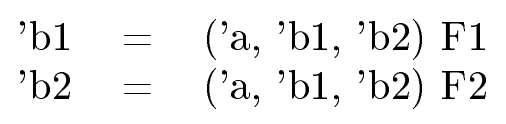
\includegraphics[width=0.3\textwidth]{img/equations.png}

\subsubsection{Encoding $F$-algebras}

Representation of algebras:

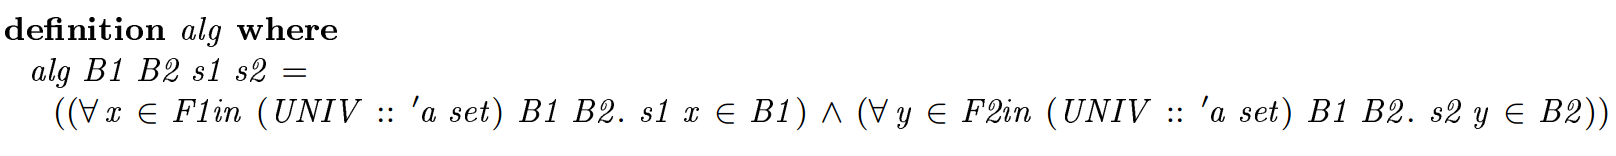
\includegraphics[width=\textwidth]{img/algebras.png}

Given morphisms $s_1: ('a, 'b, 'c) F1 \Rightarrow 'b$ and $s_2:  ('a, 'b, 'c) F2 \Rightarrow 'c$, we need to ensure that they act like structure maps on the $F$-algebra structure whose carrier set is $(B_1,B_2)$. The function Fin allows to lift from a set $S$ to the set of elements that can be built from this set using functor $S$, $F(S)$. Thus, the definition ensures that the morphisms are well-defined structure maps. 

Similarly, if one wants to specify a homomorphism $(f,g)$ between $F$-algebras $((B_1,B_2), (s_1,s_2))$ and $((B_1',B_2'), (s_1',s_2'))$ one imposes the well-definition condition on the carrier sets together with the commutativity conditions:

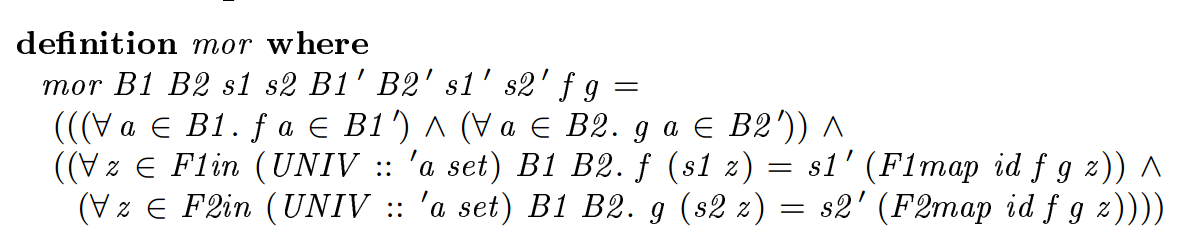
\includegraphics[width=0.7\textwidth]{img/morphisms.png}

The construction of the initial algebra happens in two stages. First one constructs  a weakly initial algebra. Then, one constructs the initial algebra from the weakly initial one. The authors systematically introduce the second step of the construction using a construction \textit{from above} of the minimal algebra generated by $\emptyset$, to then implement a construction from below that is less intuitive since it uses transfinite induction. We comment the abstract construction to precise its meaning using the remarks on subalgebras in the BNF settings that we did in the previous section. \\


\begin{construction}[Minimal algebra]
	Let $\mathcal{A}=(A,s)$ be an $F$-algebra. Set $M_s = \bigcap_{B. (B,s) \text{is a subalgebra of (A,s)}} B$ then: \[
	\mathcal{M}(\mathcal{A}) = \Big(M_s,s \Big|_{M_s} \Big)\]
	
	is the $F$-subalgebra generated by $\emptyset$.
\end{construction}	

For a formal proof that the intersection of subalgebras of a general $F$-algebra is again a subalgebra, the interested reader is referred to \cite{denecke2009universal} (theorem 5.6.5) which provides a good mathematical account of the subject. $\mathcal{A}$ is said to be the subalgebra generated by $\emptyset$ in the sense that it is the intersection of all subalgebras containing $\emptyset$. \\
	
\begin{lemma}\label{lem}
	There exists at most one morphism from $\mathcal{M}(\mathcal{A})$ to any other $F$-algebra $(Y,t)$.
\end{lemma}	
\begin{proof}
	If $f,g$ are two such morphisms, we can show that: $$B = \mathcal{M}(\mathcal{A}) \cap \{x \in \mathcal{A}. f(x) _= g(x)\}$$ is a $F$-subalgebra of $\mathcal{A}=(A,s)$
	
	Indeed, by our remarks, it suffices to note that $M_s \cap \{x \in \mathcal{A}. f(x) _= g(x)\} \subseteq M_s$ and consider the structure map $s|_B$. This leads to a subalgebra of $\mathcal{M}(\mathcal{A})$ which can be naturally seen as a subalgebra of $\mathcal{A}$. 
	
	By definition of $\mathcal{M}(\mathcal{A})$, $M_s \supseteq B$ and thus $\forall x \in M_s. f(x) = g(x)$. Thus, the morphisms are equal. 
\end{proof}
	
Here is the naive approach to the construction of an initial $F$-algebra.

\begin{enumerate}
	\item Set $\mathcal{R} = \prod \{\mathcal{A}. \mathcal{A} \text{ is an algebra}\}$.
	\item Given an algebra $\mathcal{A}$, note $h$ the projection morphism from $\mathcal{R}$ to $\mathcal{A}$.
	\item Then $h|_{\mathcal{M}(\mathcal{R})}$ is the unique morphism between $\mathcal{M}(\mathcal{R})$ and $\mathcal{A}$.
	\item Since the construction does not depend on the chosen algebra $\mathcal{A}$,  $\mathcal{M}(\mathcal{R})$ is the desired initial algebra.
\end{enumerate}

The naive approach cannot be encoded in HOL. First, one cannot quantify over infinite type collections. Second, the product of the carrier sets of all algebras, fails itself to be a set. 

Here is the enhanced naive approach to the construction of an initial $F$-algebra. Essentially, we split the construction in two phases:

Given an $F$-algebra $\mathcal{A}$ we know that there exists at most one morphism $\mathcal{M}(\mathcal{A}) \to \mathcal{A}$. But from our remarks above, for bounded natural functors, the inclusion is one such morphism. So there is exactly one morphism $g: \mathcal{M}(\mathcal{A}) \to \mathcal{A}$.

On the other hand, we would like some set of algebras $\mathcal{R}$ such that from $\mathcal{R}$ there is a unique morphism to any $\mathcal{M}(\mathcal{A})$. The strategy is two find a sufficiently large type $T_0$ such that its cardinality is an upperbound for any $\mathcal{A}$. The reason is a theorem stating that if we can bound the cardinality of a set by some ordinal then the set has a bijective representation on the carrier of the wellorder inducing the ordinal. The crucial lemma is ex\_bij\_betw:

$|A| \le_o (r :: 'b \, \text{set}) \implies \exists f \; B::'b \; \text{set}. \text{bij\_betw} f \; B \; A$

More precisely, the package shows that for all algebras $\mathcal{A}$, if $M$ denotes the carrier of $\mathcal{M}(\mathcal{A})$ then $|M| \le_o 2  \wedge_c k$. Then, the package witnesses a type $T_0$ with this cardinality and defines $\mathcal{R} = \prod \{\mathcal{A}. \mathcal{A} = (A,s) \text{ is an algebra with structure map } s: T_0 F \to T_0 \}$. By means of $ex\_bij\_betw$ the minimal algebras $\mathcal{M}(\mathcal{A})$ have isomorphic representants on a component of $\mathcal{R}$. Thus, the corresponding projection from the product to $\mathcal{M}(\mathcal{A})$ restricted to $\mathcal{M}(\mathcal{R})$ is the unique morphism  $f$ between the two. 

Then, $f \circ g: \mathcal{M}(\mathcal{R}) \to \mathcal{A}$ is a suitable morphism. One shows it is the unique morphism between the two with a similar argument as in lemma \ref{lem}.

It should be noted that the real proof does not even define $\mathcal{M}(\mathcal{A})$ as we did. Instead, the underlying construction defines the minimal algebra from below using transfinite recursion.

\subsubsection{Derived theorems and definitional framework for datatypes}

Once we understand the way in which one could compute an initial algebra of a functor, it is time to encode the proving and definitional tools that this theoretical object provides us. First we formulate the general induction principle obtained:

\begin{thm}[Induction principle of a BNF]
	Let $(\varphi_1,\dots,\varphi_n): (\overline{\alpha} IF^1,\ldots,\overline{\alpha} IF^n) \to bool$ be a tuple of predicates. Then:
	
	\[
	\infer{\forall b_1,\ldots,b_n. \varphi_1(b_1) \land \ldots \land \varphi_n(b_n)}{%
		\forall y. \forall j \in \{1,\ldots,n\}. (\bigwedge_{k = 1}^n \forall b \in \text{Fset}_{m+k}^j y. \varphi_k(b)) \implies \varphi_j(\text{fld}^j(y))
	}
	\]
\end{thm}

The package also defines iterator $iter^j$ and recursor $rec^j$ constants in a way that the following diagrams commute for each $j \in \{1,\ldots\}$. 

\begin{tikzcd}
	(\overline{\alpha},\overline{\alpha} IF^1,\ldots,\overline{\alpha} IF^n)F^j \arrow{r}{fld^j} \arrow[swap]{d}{Fmap^j \; id \ldots id \; (iter^1 s_1 \ldots s_n) \ldots (iter^n s_1 \ldots s_n)} 
	& \overline{\alpha} IF^j \arrow{d}{iter^ j s_1 \ldots s_n} \\
	(\overline{\alpha},\beta_1,\ldots,\beta_n)F^j \arrow{r}{s_j}  & \beta_j
\end{tikzcd}

\begin{tikzcd}
	(\overline{\alpha},\overline{\alpha} IF^1,\ldots,\overline{\alpha} IF^n)F^j \arrow{r}{fld^j} \arrow[swap]{d}{Fmap^j \; id \ldots id \; \langle id, rec^1 s_1 \ldots s_n \rangle \ldots \langle id, rec^n s_1 \ldots s_n \rangle} 
	& \overline{\alpha} IF^j \arrow{d}{rec^ j s_1 \ldots s_n} \\
	(\overline{\alpha},\overline{\alpha} IF^1 \times \beta_1,\ldots,\overline{\alpha} IF^n \times \beta_n)F^j \arrow{r}{s_j}  & \beta_j
\end{tikzcd}

More importantly, all this infrastructure is used in defining the BNF corresponding to the initial algebra. This allows to compose BNF's which yields the ultimate power of categorical method: the simplicity of composing its underlying constructions.

\begin{thm}
	$(IF^ j, IFmap^ j, IFset^ j, IFbd)$ defined for $j \in \{1,\ldots,n\}$ as:
	
	\begin{itemize}
		\item $\overline{\alpha} \, IF^j$ is the set constructed in the previous section.
		\item $IFmap^j: (\overline{\alpha} \to \overline{\beta}) \to (\overline{\alpha} IF^j \to \overline{\beta} IF^j)$ \\
			  $IFmap^j \, f_1 \, \ldots \, f_m = iter^j (fld^1 \circ Fmap^1 f_1 \ldots f_m \, id \ldots id) \ldots (fld^ n \circ Fmap^ n f_1 \ldots f_m \, id \ldots id)$
		\item $IFset_i^j: \overline{\alpha} \, IF^j \to \alpha_i \, set, i \in \{1,\ldots,m\}$ \\
			  $IFset_i^j = iter \, (\lambda z. Fset_i^1 z \cup \bigcup_{k=m+1}^{m+n} \cup Fset_k^1 z) \ldots (\lambda z. Fset_i^n z \cup \bigcup_{k=m+1}^{m+n} \cup Fset_k^n z)$ 
		\item $IFbd = 2^{\max\{Fbd^1,\ldots,Fbd^n\}}$
	\end{itemize}

is a BNF.
\end{thm}

Here $m$ is a parameter ensuring that the different equations share the same variables. The first $m$ occurrences are considered dead and do not play a role in this section, thus the increment by $m$ in the above formula. Also, $n$ tells the number of involved equations.

For the definition of $IFset$, we focus on the first equation:

$collect_i = \lambda z. Fset_i^1 z \cup \bigcup_{k=m+1}^{m+n} \cup Fset_k^1 z$ 

this function allows to compute the atoms of type $\alpha_i$ and then 

In the first union, we add the atoms of that variable type regardless of if it is live or not, in the rest of the union we add the atoms of the inductive components.


\begin{example}[BNF structure of lists]
	Let's see how the construction for $IFmap$ works on lists of base type $\alpha$. If we set $(\alpha,\beta)F = unit + \alpha \times \beta \, list$ then we have:

\begin{tikzcd}
	(\alpha,\alpha \, list) \arrow{r}{F(iter(s))} \arrow[swap]{d}{fld_{\alpha}} & (\alpha, \beta \, list)F \arrow{d}{Fmap \, f \, id} \arrow[bend left=90]{dd}{s} \\
	\alpha \, list \arrow[dashed,swap]{rd}{iter(s)} & (\beta, \beta \, list)F \arrow{d}{fld_{\beta}} \\
	& \beta list                                   
\end{tikzcd}


and our map function is $IFmap = iter(s) = iter(fld_{\beta} \circ Fmap \, f \, id)$. So from the mapping registered in the system there is a way to give the abstract interface $(list,map)$ of lists. 

The atoms of type $\beta$ are obtained with $Fset_1$ while onje delves into the inductive components by means of $Fset_2$:

\begin{tikzcd}
	(\beta,\beta \, IF)F \arrow[swap]{d}{fld} \arrow{r}{Fmap \, id \, IFset} &  (\beta, \beta \, set)F  \arrow{d}{collect} \\
	\beta \, IF \arrow{r}{IFset}  & \beta \, set                       
\end{tikzcd}

where $collect(a) = Fset_1(a) \cup Fset_2(a)$ and $IFset$ is defined by $IFset = iter(collect)$. 
\end{example}


\subsubsection{Encoding $F$-coalgebras}

Coge un tipo de dato coinductivo.
Formulalo como un functor.
Sigue las pruebas en GFP.

\subsubsection{Derived theorems and definitional framework for codatatypes}


\subsection{How could Stainless produce such (co)inductive principles?}

See section 2.4.4 of Jacobs coalgebras for a way of emulating coalgebras using artificial constructions. Stainless does it in a way similar to Coq with some abstract mechanism to deal with them.  

See also the images on the topic on the coinduction files under images. For the Stainless approach. 


\subsection{Basic natural functors}

Our objects are types from a type universe $U$. 

These are described theoretically in chapter 3 of \cite{traytel}. Let us take the example of the sum functor:



In /src/HOL/Tools/BNF/bnf\_def.ML we can see the definition of a bounded natural functor:

\begin{lstlisting}
	datatype bnf = BNF of {
		name: binding,
		T: typ,
		live: int,
		lives: typ list, (*source type variables of map*)
		lives': typ list, (*target type variables of map*)
		dead: int,
		deads: typ list,
		map: term,
		sets: term list,
		bd: term,
		axioms: axioms,
		defs: defs,
		facts: facts,
		nwits: int,
		wits: nonemptiness_witness list,
		rel: term,
		pred: term
	};
\end{lstlisting}

as a datatype constructor with only one sort which takes a record as a parameter. 

Some examples of how to build and proof a BNF correct can be found in /src/HOL/Basic\_BNFs.thy


Construction of an initial algebra from a weakly initial algebra

Let $\mathcal{A} = (A,s)$ be an algebra.

Let $M_s$ be the intersection of all sets $B$ such that $(B,s)$ is an algebra.

It seems evident that if we understand the minimal algebra generated by $\mathcal{A}$, $M(\mathcal{A})$ as a subalgebra, such that any other subalgebra is a subalgebra of this one.

Statement 1: $\mathcal{M}(\mathcal{A}) = (M_s,s)$

Statement 2: there exists at most one morphism from $M(\mathcal{A})$ to any other algebra...

Statement 3: given a weakly initial algebra $\mathcal{C}$, the desired initial algebra is its minimal subalgebra $\mathcal{M}(\mathcal{C})$ 





\section{Applications}

e-voting system
other consensus
termination

\newpage
\printbibliography





\end{document}